% Appendix A

\chapter{Distribuciones estadísticas en Telecomunicaciones} % Main appendix title

\label{AppendixA} % For referencing this appendix elsewhere, use \ref{AppendixA}

El objetivo de este apéndice fue revisar las distribuciones de probabilidad mas utilizadas en los sistemas de comunicaciones móviles para caracterizar los fenómenos más importantes en este ámbito, después se describió la implementación y puesta a prueba de la generación de las variables aleatorias utilizadas en el simulador, esto con el fin de brindar fiabilidad en los resultados obtenidos.\newline

%----------------------------------------------------------------------------------------
%	SECTION 1
%----------------------------------------------------------------------------------------

El uso de modelos estadísticos es importante para describir diferentes fenomenos en el campo de las telecomunicaciones\parencite{Correia2018}:
\begin{itemize}
    \item Llamadas telefónicas y conexiones de datos
    \item Influencia del usuario en el rendimiento de la red
    \item Propagación no guiada en ambientes aleatorios
    \item Movilidad del usuario
\end{itemize}

Comúnmente se utilizan las siguientes distribuciones de probabilidad en telecomunicaciones \parencite{Correia2018}:

\begin{enumerate}
    \item Distribución Uniforme: Es usada para describir la fase de una señal. También, se ha utilizado para simular el despliegue de BSs \parencite{TurjmanSmallCells}.
    \item Distribución Normal (Gaussiana): Es usada para describir fluctuaciones alrededor de un valor medio, p.ej. \textit{shadowing}. Esta distribución no puede ser usada para describir entidades que no pueden ser negativas.
    \item Distribución Log-Normal: Es usada para describir entidades como la potencia de una señal, amplitudes, principalmente el desvanecimiento lento.
    \item Distribución Rayleigh: Es usada para describir el desvanecimiento rápido-intenso.
    \item Distribución Susuki: Describe conjuntamente el desvanecimiento lento y rápido.
    \item Distribución Rice: Es usada para describir el desvanecimiento rápido - no-intenso.
    \item Distribución Exponencial: Es ampliamente usada para describir la duración de diferentes fenómenos, principalmente asociados con el desvanecimiento de señales y las llamadas telefónicas.
    \item Distribución de Bernoulli: Es usada para describir la ocupación de canales de telecomunicaciones.
    \item Distribución binomial: Es usada para describir llamadas telefónicas.
\end{enumerate}

\section{Generación de números aleatorios}

La distribución uniforme (también llamada distribución rectangular) es una familia de curvas de dos parámetros que es notable porque tiene una función de distribución de probabilidad constante (PDF) entre sus dos parámetros delimitadores. La distribución uniforme se utiliza en técnicas de generación de números aleatorios, como el método de inversión \parencite{ UniformMatlab}.\newline

Se puede usar la distribución uniforme estándar para generar números aleatorios para cualquier otra distribución continua mediante el método de inversión. El método de inversión se basa en el principio de que las funciones de distribución acumulativa continua (CDFs) varían uniformemente durante el intervalo abierto $(0, 1)$ . Si $u$ es un número aleatorio uniforme en (0, 1) , entonces $x = F^{ -1} ( u )$ genera un número aleatorio $x$ a partir de la distribución continua con la CDF especificada $F$ \parencite{UniformMatlab}.\newline

En teoría de la probabilidad y estadística, hay varias relaciones entre las distribuciones de probabilidad. Estas relaciones se pueden clasificar en los siguientes grupos \parencite{univariateDist}:
\begin{itemize}
    \item Una distribución es un caso especial de otra con un espacio de parámetros más amplio.
    \item Transformaciones (función de una variable aleatoria).
    \item Combinaciones (función de varias variables).
    \item Relaciones de aproximación (límite).
    \item Relaciones compuestas (útiles para la inferencia bayesiana [\textit{Bayesian inference}]).
\end{itemize}

\begin{figure}[th]
    \centering
    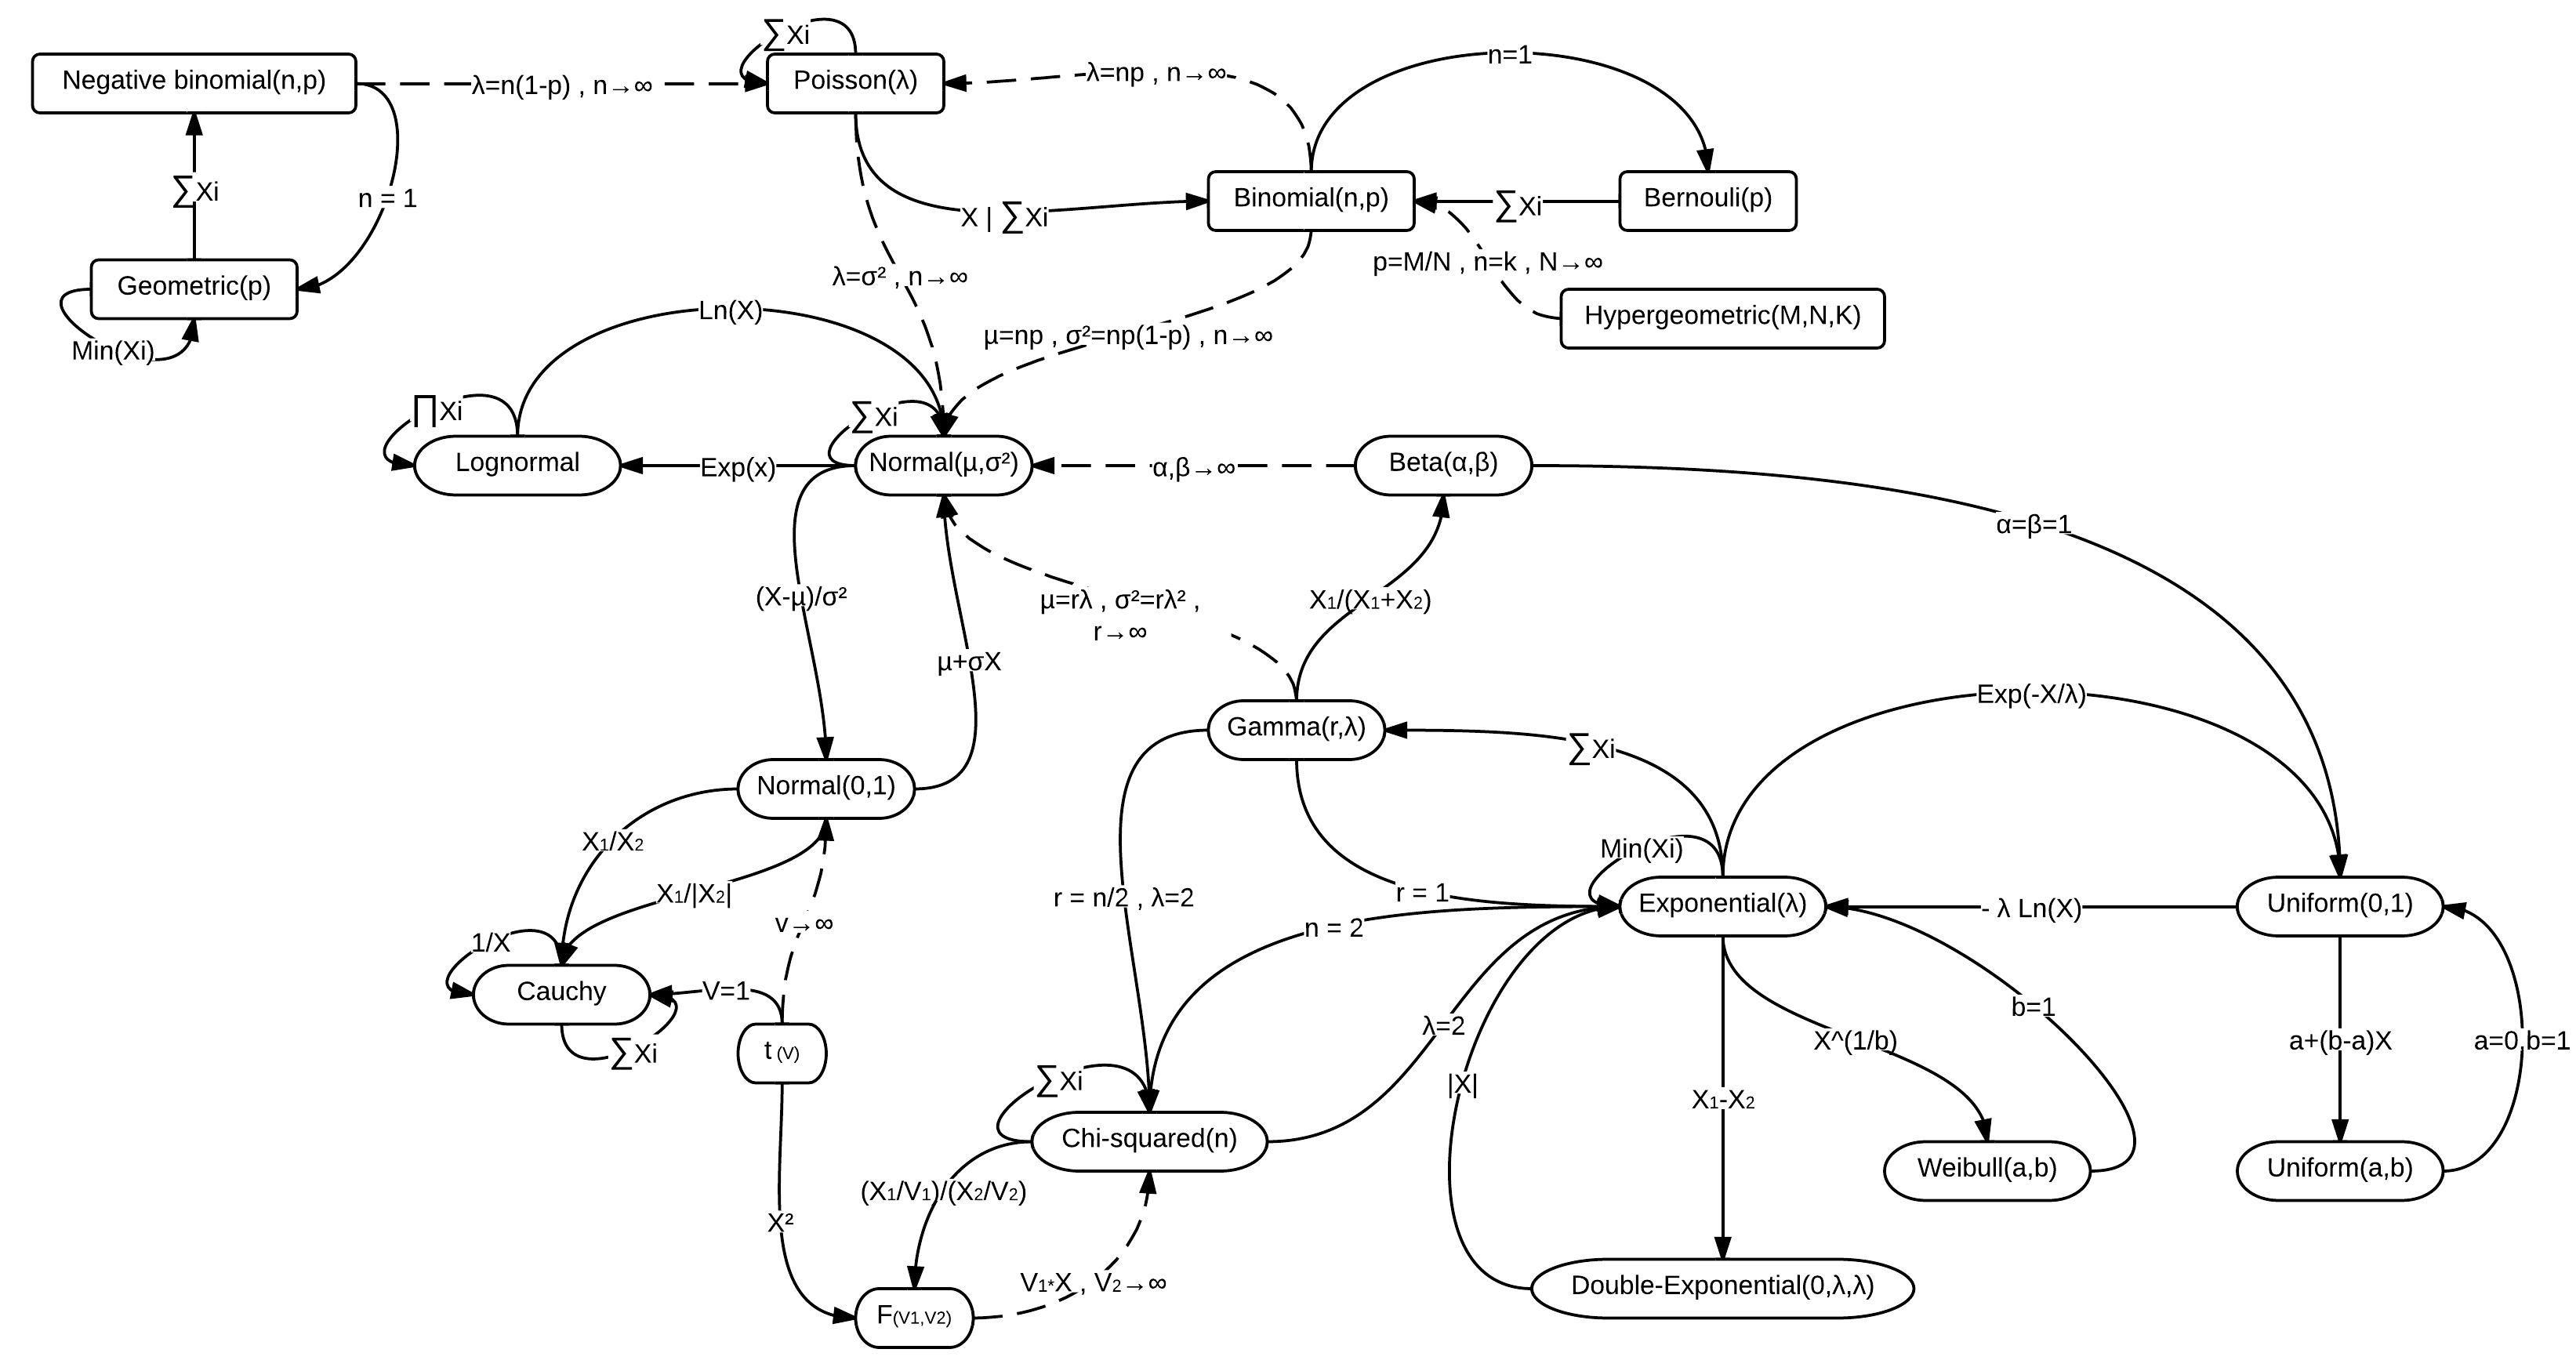
\includegraphics[scale=0.63]{Figures/RelacionesProbabilidad}
    \decoRule
    \caption[Relaciones entre algunas de las distribuciones de probabilidad univariadas]{Las relaciones entre algunas de las distribuciones de probabilidad univariadas se ilustran con líneas conectadas, las líneas discontinuas significan relación aproximada. [Fuente: \parencite{univariateDist}]}
    \label{fig:relacionesDistribuciones}
\end{figure}

\break

\section{Generación de distribuciones estadísticas para el simulador}

\subsection{Generación de variable aleatoria tipo \textit{Poisson}}
Como se revisó en la sección~\ref{generarGeoEstocastica}, uno de los requisitos para generar una geometría estocástica es que el número de puntos en el plano sea Poisson, es por esto que en esta sección se comprobó la generación de la variable aleatoria Poisson en Python usando la libreria \textit{scipy}.\newline

Para esto, se realizaron $10000$ generaciones de numeros siguiendo una distribución de Poisson con tasa $\lambda = 20$, se obtuvo el histograma de todos los números generados y se comparó con su función de masa de probabilidad (PMF).\newline

Se observa que la distribución del histograma sigue a la función masa de probabilidad de Poisson [\textit{véase Figura~\ref{fig:generacionPoisson}}], por lo que se valida la generación de números Poisson en Python.\newline

\begin{figure}[th]
    \centering
    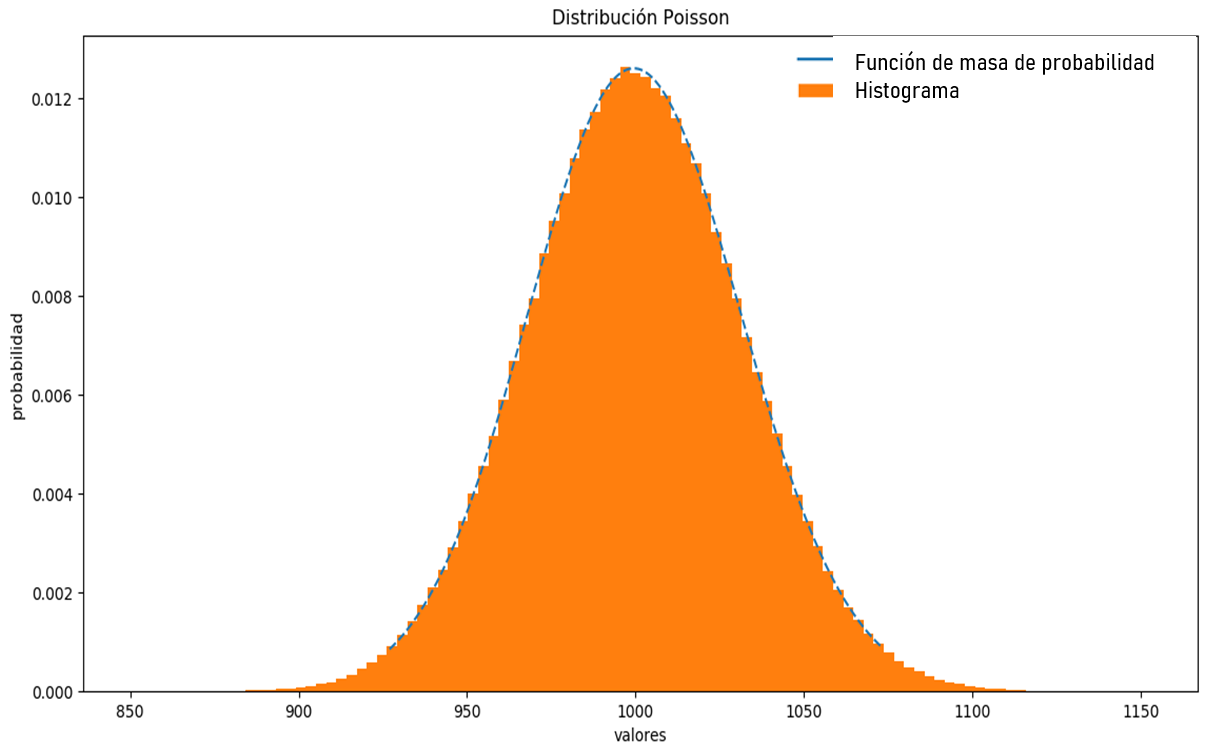
\includegraphics[scale=.5]{Figures/PoissonDistribution}
    \decoRule
    \caption[Gráfica comparación PMF e histograma de distribución Poisson en Python]{Gráfica comparación PMF e histograma de distribución Poisson en Python}
    \label{fig:generacionPoisson}
\end{figure}
\break

\subsection{Generación de variables aleatorias tipo \textit{Exponencial} y \textit{Rayleigh}}

Como se revisó en la sección~\ref{DesvRayleigC2}, cuando el desvanecimiento es de tipo Rayleigh, la magnitud o amplitud de la señal es Rayleigh y la potencia es exponencial. En esta sección, se comprobó la generación de estas variables aleatorias en Python usando la libreria \textit{random}.\newline

Se realizaron $10000$ generaciones de numeros siguiendo una distribución Exponencial negativa con media $\mu =1$, se obtuvo el histograma de todos los números generados y se comparó con su función de densidad de probabilidad (PDF).\newline

De la misma manera con la otra distribución, se realizaron $10000$ generaciones de numeros siguiendo una distribución Rayleigh con desviación estándar $\sigma = 1$, se obtuvo el histograma de todos los números generados y se comparó con su función de densidad de probabilidad (PDF).\newline

Se observa que la distribuciones de los histogramas siguen a su respectiva función densidad de probabilidad (PDF) [\textit{véanse Figuras~\ref{fig:generacionExpon} y \ref{fig:generacionRay} }], por lo que se valida la generación de números Exponenciales y Rayleigh en Python.\newline

\begin{figure}[th]
    \centering
    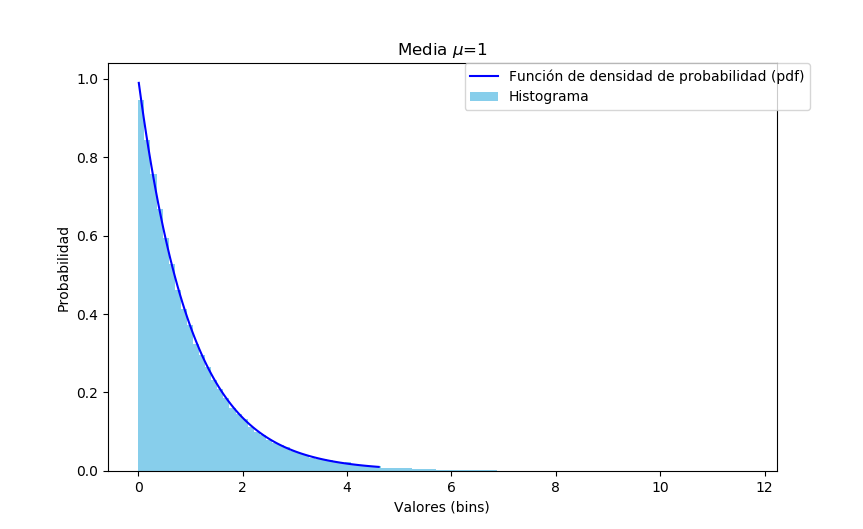
\includegraphics[scale=.6]{Figures/ExponentialDisitribution.png}
    \decoRule
    \caption[Gráfica comparación PDF e histograma de distribución Exponencial en Python]{Gráfica comparación PDF e histograma de distribución Exponencial en Python}
    \label{fig:generacionExpon}
\end{figure}

\begin{figure}[th]
    \centering
    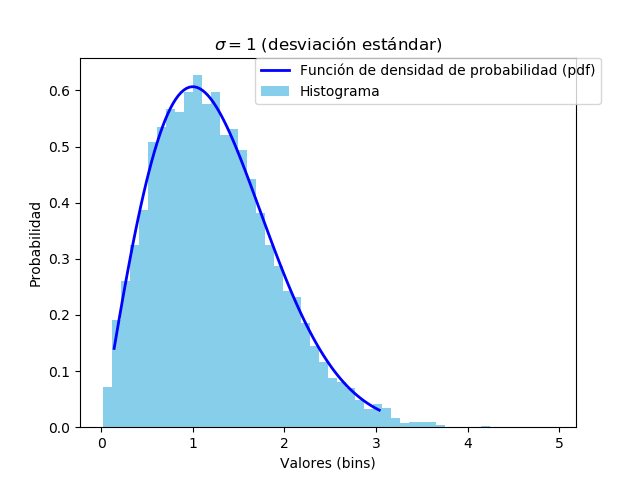
\includegraphics[scale=.7]{Figures/RayleighDistribution.png}
    \decoRule
    \caption[Gráfica comparación PDF e histograma de distribución Rayleigh en Python]{Gráfica comparación PDF e histograma de distribución Rayleigh en Python}
    \label{fig:generacionRay}
\end{figure}
\break

\subsection{Generación de variable aleatoria tipo \textit{Pareto}}

Como se revisó en la sección~\ref{Informesperiodicos}, la longitud de paquetes en la transmisión periodica siguió una distribución de Pareto con parámetro alfa = 2.5 y tamaño mínimo de carga útil de la aplicación = 20 bytes con un corte a 200 bytes.\newline

La distribución de Pareto a veces se conoce como el Principio de Pareto o la regla '80 –20 ', en este caso la regla establece que el 80\% de los tamaños de paquete que se formarán, los producirán solo el 20\% de los dispositivos del sistema y viceversa.\newline

La distribución de Pareto se puede replicar en Python usando el módulo Scipy.stats o NumPy. El módulo Scipy.stats abarca varias distribuciones de probabilidad y una biblioteca cada vez mayor de funciones estadísticas. Se comprobó la generación de esta variable aleatoria en Python usando la libreria \textit{scipy}.\newline

Se realizaron $100000$ generaciones de numeros siguiendo una distribución areto con parámetro alfa  $\alpha =2.5$ acotada entre 20 y 200, se obtuvo el histograma de todos los números generados y se comparó con su función de densidad de probabilidad (PDF).\newline

Se observa que la distribución del histograma sigue a la función densidad de probabilidad Pareto [\textit{véase Figura~\ref{fig:generacionPareto}}], por lo que se valida la generación de números Pareto en Python.\newline

\begin{figure}[th]
    \centering
    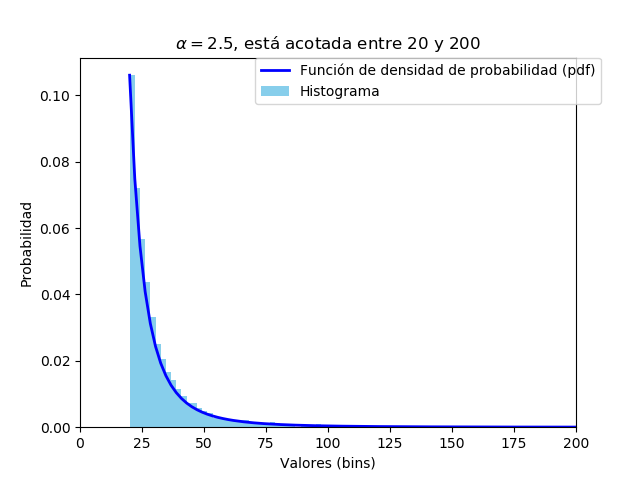
\includegraphics[scale=.7]{Figures/ParetoDIstribution}
    \decoRule
    \caption[Gráfica comparación PDF e histograma de distribución Pareto en Python]{Gráfica comparación PDF e histograma de distribución Pareto en Python}
    \label{fig:generacionPareto}
\end{figure}

